\documentclass[a4paper]{article}

\usepackage[margin=0.5cm]{geometry}
\usepackage{qtree}
\usepackage{color}
\usepackage{forest}
\usepackage{tikz}
\usepackage{listings}

\begin{document}
\begin{titlepage}
	\begin{center}
		\begin{figure}[t]
			\centering
			
\includegraphics[width=350px]{logo.PNG}
		\end{figure}
		
		\begin{center}
			\textsc{\Huge Programming Languages}
		\end{center}
		\begin{center}
			\textsc{\Huge COS 333}
		\end{center}
		\begin{center}		
			\textsc{\LARGE Practical Lab Experience 1:}		
		\end{center}
		\begin{center}		
			\textsc{\LARGE Research Assignment}		
		\end{center}
		
		\begin{flushright} \large
			Juan Jaques du Preez \newline \emph{u15189016} \newline
		\end{flushright}
\par\vspace{\fill}
{\large Date:}
\\
{\large \today}

	\end{center}
\end{titlepage}

\tableofcontents
\newpage

\section{Overview}
	\subsection{Overall UML Diagram}
		\begin{center}
			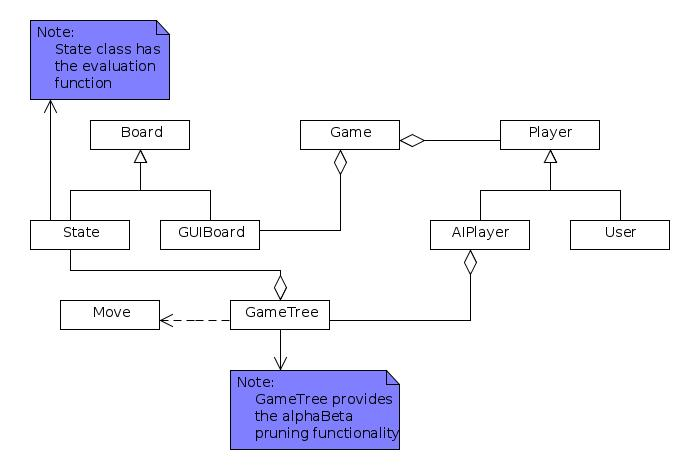
\includegraphics[width=350px]{fullUML.jpg}	
		\end{center}
	
	\subsection{Game Choice}
	I have decided to go with the \textsc{\LARGE Boa} game, because it seemed like more of a challenge.
	\subsection{Algorithm Choice}
	I chose to have \textsc{\LARGE alphaBeta pruning} functionality instead of just a simple minimax. The function itself and its 
	description is at the end of the document. The function can also be found in the GameTree.cpp file.
\section{Compile and Run Program}
\section{Evaluation Function}
	\subsection{the function}
	This function can be found in the State.cpp file:
	\begin{lstlisting}
int State::evaluate(bool player)
{
	//calculate if losing position 100 or -100
	if (isLosingPosition())
	{
		if (favouredPlayer == player)
			return 100;
		else return -100; 
	}
	
	//weights
	const float countSeedWeight = 30.0/100;
	const float frontRowWeight = 20.0/100;
	const float backRowWeight= 10.0/100;
	const float frontRowOccWeight = 15.0/100;
	const float backRowOccWeight= 5.0/100;
	const float captureWeight = 20.0/100;
	
	
	//count seeds for each player
	int countSeed;
	int p1 = 0;
	for (int i = 0; i < 8; i++)
	{
		p1 += board[2][i] + board[3][i];
	}
	int p2 = 0;
	for (int i = 0; i < 8; i++)
	{
		p2 += board[0][i] + board[1][i];
	}
	if (player == PLAYER1) countSeed = (p1 - p2);
	else countSeed = (p2 - p1);
	
	//count seeds in front rows and back rows respectively
	int frontRow;
	int backRow;
	p1 =0;
	int p1b = 0;
	for (int i = 0; i < 8; i++)
	{
		p1 += board[2][i];
		p1b += board[3][i];		
	}
	p2 = 0;
	int p2b = 0;
	for (int i = 0; i < 8; i++)
	{
		p2 += board[1][i];
		p2b += board[0][i];
	}
	if (player == PLAYER1) 
	{
		frontRow = p1 - p2;
		backRow = p1b - p2b;
	}
	else 
	{
		frontRow = p2 - p1;
		backRow = p2b - p1b;
	}		
	
	//count how many holes are occupied in back row and front rows
	int frontRowOcc;
	int backRowOcc;
	p1 =0;
	p1b = 0;
	for (int i = 0; i < 8; i++)
	{
		if (board[2][i] != 0) p1++;
		if (board[3][i] != 0) p1b++;
	}
	p2 = 0;
	p2b = 0;
	for (int i = 0; i < 8; i++)
	{
		if (board[1][i] != 0) p2++;
		if (board[0][i] != 0) p2b++;
	}	
	if (player == PLAYER1) 
	{
		frontRowOcc = p1 - p2;
		backRowOcc = p1b - p2b;
	}
	else 
	{
		frontRowOcc = p2 - p1;
		backRowOcc = p2b - p1b;
	}	
	
	//count the number of seeds each player can capture
	int capture = 0;
	p1 =0;
	p2 = 0;
	for (int i = 0; i < 8; i++)
	{
		if (board[2][i] != 0 && board[1][i])
		{
			p1 += board[1][i];
			p2 += board[2][i];
		}
	}
	if (player == PLAYER1) capture = p1 - p2;
	else capture = p2 - p1;
	
	//return weighted sum
	return countSeedWeight * countSeed
		+ frontRowWeight * frontRow
		+ backRowWeight * backRow		
		+ frontRowOccWeight * frontRowOcc
		+ backRowOccWeight * backRowOcc
		+captureWeight * capture;
}
	\end{lstlisting}

	\subsection{Description of Evaluation function}
	In this function, there are six different aspects of a particular board state that I considered. Each of these six 
	apects are then multiplied with a pre-determined weight which I have assigned to them based on how important I think the 			step is.  Notice that each of these aspects can be zero or negative, thus giving a total evaluation number which is always 
	between -100 and 100. These six aspects are described as follows:
	\subsubsection{the number of seeds on each side of the board}
	The function simple counts the number of seeds on each player's side and subtracts the opponent's total number
	from the current player's total number of seeds.
	\subsubsection{the number of seeds in each front row}
	The same is then done for the first row or top row of each player. This is done because the front row seeds are more 
	valuable than those in the back row.
	\subsubsection{the number of seeds in each back row}
	These back row seeds still have some value and also need to be calculated.
	\subsubsection{the distribution of seeds in each front row}
	This part of the function counts how many non-empty holes there are in the front row and gives it in a ratio of x/8. This
	is done to see how distributed the seeds are. It is not helpful when you have 20 seeds, but they are all accumulated in
	a single hole. At the end, these two values are subtracted from one another.
	\subsubsection{the distribution of seeds in each back row}
	This is then done for the bottom hole as well.
	\subsubsection{possible captures}
	The total number of seeds that can a player can capture is summed up for each player. Then the difference is taken again. 
	

\section{AlphaBeta pruning function}
\begin{lstlisting}
\end{lstlisting}

\end{document}
